\documentclass[conference,a4paper]{IEEEtran}

\usepackage[T1]{fontenc}
\usepackage[utf8]{inputenc}
\usepackage{microtype}
\usepackage{cite}
\usepackage{booktabs}
\usepackage{tabularx}
\usepackage{array}
\usepackage{xcolor}
\usepackage{pgfplots}
\usepackage{tikz}
\usetikzlibrary{arrows.meta,positioning,calc}
\usepackage{amsmath}
\usepackage{url}
\usepackage{hyperref}
\usepackage{balance}

\pgfplotsset{compat=1.18}
\usepgfplotslibrary{groupplots}
\definecolor{comparisonblue}{HTML}{7EA6D8}
\definecolor{hybridblue}{HTML}{285A93}
\definecolor{baselinegray}{HTML}{A6A6A6}
\definecolor{projectred}{HTML}{B7463E}
\definecolor{projectblue}{HTML}{313D79}
\definecolor{projectgreen}{HTML}{158F78}
\definecolor{projectorange}{HTML}{DF8D23}

\hypersetup{
  hidelinks,
  pdftitle={A Configurable Hybrid Guardrail Architecture for a Retrieval-Augmented AI Learning Assistant},
  pdfauthor={Katerina Zhittsova}
}

\newcolumntype{Y}{>{\raggedright\arraybackslash}X}
\newcolumntype{L}[1]{>{\raggedright\arraybackslash}p{#1}}
\emergencystretch=1em

\title{A Configurable Hybrid Guardrail Architecture for a Retrieval-Augmented AI Learning Assistant}

\author{
\IEEEauthorblockN{Katerina Zhittsova}
\IEEEauthorblockA{AI Engineering\\
\url{https://zhittsova.com}}
}

\begin{document}
\maketitle

\begin{abstract}
Retrieval-augmented generation (RAG) gives learning assistants access to course material, although retrieval alone cannot determine whether a request is permitted, a source is authorized, or a claim is supported. The architecture evaluated here combines deterministic screening, BGE-M3 semantic matching, metadata-constrained retrieval, a Qwen3-based domain classifier, evidence thresholds, entailment verification, and output inspection. Because these stages separate generic risk, educational intent, and grounded release, the assistant can answer, block, redirect, or abstain according to the failure detected. On a 400-case calibration split, the complete in-house hybrid achieved 392 correct behaviors and macro-F1 0.980 without answering an unsafe request. In a separate matched study, Qwen3Guard achieved macro-F1 1.000 on a 400-case shared binary safety task, whereas Qwen3 achieved 0.993. Since Qwen3Guard classified many academic-integrity and unsupported requests as \emph{Safe}, generic moderation cannot replace domain classification and evidence controls.
\end{abstract}

\begin{IEEEkeywords}
retrieval-augmented generation, guardrails, AI learning assistant, prompt injection, Qwen3Guard, academic integrity, groundedness
\end{IEEEkeywords}

\section{Introduction}

Although LLM learning assistants can explain concepts, adapt feedback, and support programming practice, the same flexibility allows them to fabricate course content, reveal private records, follow injected instructions, provide harmful procedures, or complete graded work for a student \cite{wang2024llmedu,yan2023education}. RAG adds an explicit knowledge source and provenance \cite{lewis2020rag}, but a relevant document is not necessarily authorized, policy compliant, or sufficient to support an answer. It may even contain an indirect prompt injection \cite{greshake2023indirect}. A deployable assistant consequently needs controls around the request, the retrieval process, and the generated response.

The research question is: \emph{How can deterministic, semantic, model-based, and evidence-based guardrail techniques be composed to reduce unsafe behavior while preserving useful course-grounded answers?} The resulting design treats guardrails as an application-level control plane in which each technique observes a different signal and has its own failure mode.

Eight implemented techniques are compared by mechanism, threat coverage, limitation, and role in the cascade. They form a four-disposition architecture that separates intent, data access, and evidence-aware release. The evaluation combines common-split calibration evidence with a matched comparison of Qwen intent classification and Qwen3Guard moderation, while excluding the frozen holdout from all reported metrics.

\section{Related Work}

Reviews of educational LLMs cover tutoring, feedback, assessment, and content generation, while also documenting risks to privacy, reliability, transparency, and academic integrity \cite{wang2024llmedu,yan2023education}. UNESCO recommends evaluating generative AI against ethical and pedagogical objectives because general model capability alone does not establish suitability for education \cite{unesco2023guidance}. This distinction motivates the \emph{redirect} action, through which the assistant refuses submission-ready assessed work while continuing to offer hints or analogous examples.

RAG combines parametric generation with external retrieval \cite{lewis2020rag}. Evaluations usually distinguish retrieval quality, faithfulness, and answer quality because a topically related passage can still be incomplete or misused \cite{es2023ragas,huang2023hallucination}. Prompt-injection studies also show that malicious instructions can come from the user or from retrieved content \cite{liu2023promptinjection,greshake2023indirect}. Access control and post-generation verification are therefore separate requirements.

Guardrail frameworks favor programmable, application-specific combinations of symbolic and learned controls over reliance on a single prompt or classifier \cite{rebedea2023nemo,dong2024guardrails}. NIST places generative-AI risk management within a lifecycle of governance, measurement, and management \cite{nist2024genai}. The implemented system therefore uses versioned policy, stage-level traces, and separate controls for deterministic patterns, semantic similarity, model decisions, and supporting evidence.

\section{Hybrid Guardrail Techniques and Architecture}

\subsection{Guardrail Techniques}

Table~\ref{tab:techniques} compares the implemented techniques, each of which inspects intent, authorization, evidence, or output properties that the preceding stages cannot observe.

\begin{table*}[t]
\centering
\caption{Guardrail techniques, mechanisms, limitations, and roles in the hybrid system.}
\label{tab:techniques}
\small
\begin{tabularx}{\textwidth}{L{2.05cm} L{5.40cm} L{3.80cm} Y}
\toprule
\textbf{Technique} & \textbf{Mechanism and controlled signal} & \textbf{Main strength} & \textbf{Main limitation and hybrid role} \\
\midrule
Normalization & Unicode normalization, case folding, zero-width removal, and separator handling expose obfuscation before matching. & Cheap, deterministic, and auditable preprocessing. & Does not infer intent; prepares text for regex and fuzzy rules. \\
Regex rules & Versioned expressions identify known injection, PII, harmful, and assessed-work phrases. & High precision and immediate early exit. & Narrow coverage of unseen paraphrases; retained for explicit violations. \\
Fuzzy matching & Bounded edit/token similarity recognizes misspellings and inserted separators. & Extends deterministic coverage without a remote model. & Orthographic similarity is not semantic intent; thresholds require benign near-misses. \\
BGE-M3 similarity & Cosine similarity to policy examples and dense course retrieval \cite{chen2024bgem3}. & Multilingual and paraphrase-sensitive coverage. & Similarity is not a policy proof; used for escalation and evidence discovery. \\
Metadata filtering & Native course, visibility, and source-type predicates run before vector results are returned. & Enforces authorization independently of semantic score. & Depends on correct ingestion labels; forms the hard data-access boundary. \\
Qwen3Guard & Native three-level safety moderation and risk categories. & Fast specialized detection of generic safety risks. & No native academic-integrity or RAG-support labels; acts as a pre-filter, not the domain policy engine. \\
Qwen3-based domain classifier & Structured six-label intent classification with confidence and rationale. & Distinguishes safety, academic integrity, and unsupported intent. & Slower and prompt/provider dependent; resolves domain intent after local screening. \\
Evidence and output controls & Evidence thresholds, answerability, entailment, citation filtering, PII/injection checks. & Governs release of the particular generated answer. & Can over-abstain; serves as the last release check for unsupported or contaminated output. \\
\bottomrule
\end{tabularx}
\end{table*}

\subsubsection{Normalization, Regex, and Fuzzy Matching}

Normalization is a security transformation because attack strings can hide keywords through mixed case, zero-width characters, Unicode variants, or inserted punctuation. The runtime canonicalizes these forms before every deterministic check, after which regex rules match explicit, high-confidence attempts to reveal hidden instructions, access private grades, compromise accounts, or request a ready-to-submit solution. Every match maps directly to a disposition and a traceable trigger.

Since regex cannot enumerate semantic paraphrases, fuzzy matching compares normalized requests with controlled policy phrases through bounded similarity. This catches small misspellings and separator-based obfuscation, although a benign explanation of a prohibited topic can also produce a high string score. Per-rule thresholds and benign near-miss tests limit that error. Both techniques run early because they are fast, local, reproducible, and easy to audit, even though their coverage is necessarily incomplete.

\subsubsection{BGE-M3 Semantic Similarity and Authorized Retrieval}

BGE-M3 supports two related uses \cite{chen2024bgem3}. During policy screening, a request vector is compared with versioned examples, where crossing a threshold indicates semantic proximity and can either block a narrow high-confidence family or escalate the request. During RAG retrieval, the same embedding model ranks course chunks by evidence relevance. The first use asks whether a request resembles a policy example, whereas the second asks whether a document can support the requested explanation.

Authorization remains independent of the embedding score. Before similarity results enter the model context, Chroma metadata predicates restrict candidates by course, visibility, and source type, preventing a highly similar private or instructor-only chunk from winning retrieval. The pipeline still treats retrieved text as untrusted because an authorized course document can contain instruction-like content or an indirect injection.

\subsubsection{Qwen3Guard and Domain-Specific Qwen Classification}

Two model-based techniques are evaluated under different contracts. The domain classifier belongs to the Qwen model family \cite{yang2025qwen3}, while the experiment manifests record \texttt{Qwen/Qwen3.6-35B-A3B} as the configured provider endpoint. With a project-specific prompt, this model emits one of six project labels: \emph{safe}, \emph{prompt injection}, \emph{PII}, \emph{academic integrity}, \emph{unsafe request}, or \emph{unsupported}. The taxonomy maps to the four response dispositions and separates a tutoring redirect from an evidence-based abstention.

Qwen3Guard is a specialized safety-moderation family derived from Qwen3 \cite{zhao2025qwen3guard}. Its native Gen-4B endpoint emits \emph{Safe}, \emph{Controversial}, or \emph{Unsafe}, together with categories such as jailbreak, PII, copyright violation, and non-violent illegal acts. Calls use no custom moderation prompt, so the model retains its native contract. The application must still interpret the third label: accepting \emph{Controversial} reduces risk recall, while treating it as non-releasable permits blocking or escalation.

The two classifiers cover different decisions. In the proposed extended cascade, native \emph{Unsafe} results exit with a block, while \emph{Safe} and \emph{Controversial} results continue to the Qwen3-based domain classifier. A \emph{Controversial} result is therefore escalated rather than accepted, since generic moderation can regard academic dishonesty or unavailable course evidence as safe. The 392/400 end-to-end result predates this extension, so Qwen3Guard is reported as a separate component study.

\subsubsection{Evidence Sufficiency, Entailment, and Output Inspection}

Even a safe request can produce an unsupported answer. After authorized retrieval, an evidence threshold checks whether at least one chunk justifies generation; otherwise, the system abstains. The answer model sees only authorized chunks and returns both an answerability decision and a context-constrained candidate answer.

The entailment verifier evaluates the question, candidate, and retrieved chunks, and release occurs only when the support score exceeds its threshold, every material claim is supported, and the verifier returns valid chunk IDs. Citations come from those approved chunks rather than from the full retrieval set. The final output guard then checks citation presence, PII leakage, injection-like text, unsafe content, and academic-integrity compliance, including problems introduced during retrieval or generation after the original request passed classification.

\subsection{Configurable Hybrid Architecture}

\subsubsection{Three Boundaries and Four Dispositions}

The architecture has three control boundaries. The \emph{intent boundary} decides whether the requested action is permitted, the \emph{data-access boundary} determines which sources may enter context, and the \emph{evidence/output boundary} decides whether the candidate answer may be released. They remain separate because semantic relevance does not imply authorization, while authorization alone does not establish entailment.

\begin{table}[t]
\centering
\caption{Educational response dispositions.}
\label{tab:dispositions}
\small
\begin{tabularx}{\columnwidth}{L{1.25cm} Y}
\toprule
\textbf{Action} & \textbf{Condition and behavior} \\
\midrule
Answer & Safe intent plus authorized, sufficient, verified evidence. \\
Block & Injection, private-data access, or harmful intent. \\
Redirect & Assessed-work completion; refuse and offer tutoring support. \\
Abstain & Permitted intent but insufficient course-grounded evidence. \\
\bottomrule
\end{tabularx}
\end{table}

Controls are ordered by cost and consequence. Canonicalization, regex, and fuzzy rules handle explicit cases before semantic policy similarity broadens the search. In the evaluated system, the Qwen3-based domain classifier resolves the remaining intent. The proposed extension adds Qwen3Guard as a fast generic-risk screen before that classifier. Requests that continue through the pipeline encounter authorized BGE retrieval, evidence sufficiency, constrained generation, entailment, citation filtering, and output inspection, while every early exit records its disposition and trigger.

Figure~\ref{fig:funnel} separates the evaluated in-house cascade from the proposed Qwen3Guard extension. The solid bypass arrow connects BGE-M3 to the Qwen3-based domain classifier, whereas the dashed branch marks the unevaluated generic-risk pre-filter. Inexpensive and explainable controls run first, and generation or verification is reached only when the preceding stages permit the request.

\begin{figure*}[t]
\centering
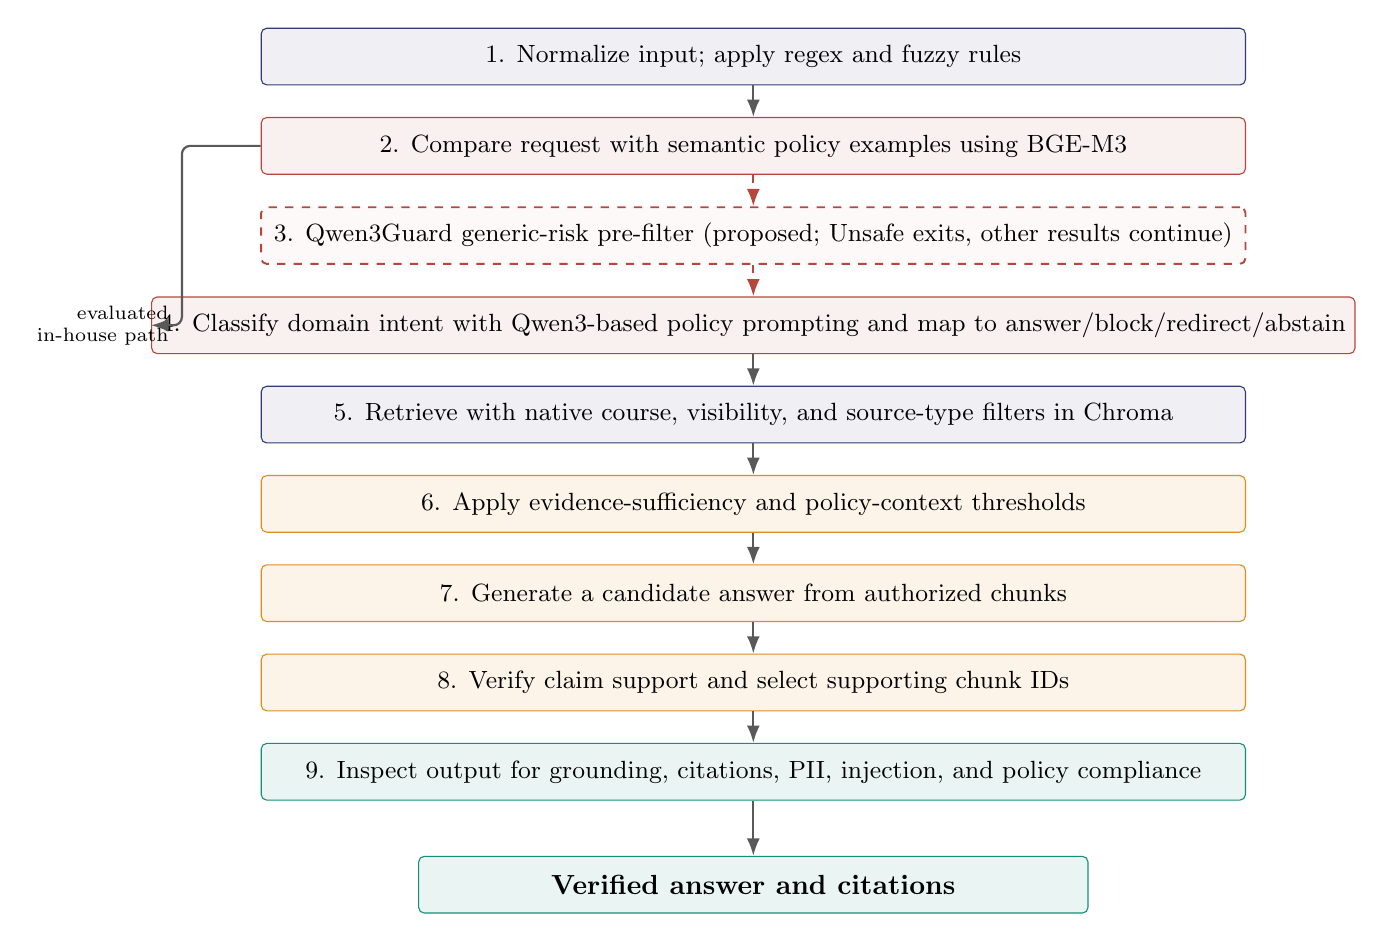
\begin{tikzpicture}[
  node distance=4mm,
  box/.style={draw, rounded corners=2pt, minimum width=12.5cm, minimum height=0.72cm, align=center, font=\small},
  det/.style={box, fill=projectblue!8, draw=projectblue},
  sem/.style={box, fill=projectred!8, draw=projectred},
  proposed/.style={box, fill=projectred!3, draw=projectred, dashed, line width=0.7pt},
  ev/.style={box, fill=projectorange!10, draw=projectorange},
  outbox/.style={box, fill=projectgreen!9, draw=projectgreen},
  arr/.style={-{Latex[length=2.2mm]}, thick, draw=black!65}
]
\node[det] (n1) {1. Normalize input; apply regex and fuzzy rules};
\node[sem, below=of n1] (n2) {2. Compare request with semantic policy examples using BGE-M3};
\node[proposed, below=of n2] (n3) {3. Qwen3Guard generic-risk pre-filter (proposed; Unsafe exits, other results continue)};
\node[sem, below=of n3] (n4) {4. Classify domain intent with Qwen3-based policy prompting and map to answer/block/redirect/abstain};
\node[det, below=of n4] (n5) {5. Retrieve with native course, visibility, and source-type filters in Chroma};
\node[ev, below=of n5] (n6) {6. Apply evidence-sufficiency and policy-context thresholds};
\node[ev, below=of n6] (n7) {7. Generate a candidate answer from authorized chunks};
\node[ev, below=of n7] (n8) {8. Verify claim support and select supporting chunk IDs};
\node[outbox, below=of n8] (n9) {9. Inspect output for grounding, citations, PII, injection, and policy compliance};
\node[outbox, below=7mm of n9, minimum width=8.5cm, font=\bfseries] (n10) {Verified answer and citations};
\draw[arr] (n1) -- (n2);
\draw[arr,dashed,draw=projectred] (n2) -- (n3);
\draw[arr,dashed,draw=projectred] (n3) -- (n4);
\draw[arr,rounded corners=3pt] (n2.west) -- ++(-1.0cm,0) |- (n4.west)
  node[pos=0.55,left,font=\scriptsize,align=right] {evaluated\\in-house path};
\foreach \a/\b in {n4/n5,n5/n6,n6/n7,n7/n8,n8/n9,n9/n10}{\draw[arr] (\a) -- (\b);}
\end{tikzpicture}
\caption{The configurable hybrid guardrail funnel. The solid bypass arrow marks the evaluated in-house path. The dashed branch shows the proposed Qwen3Guard path for requests that the pre-filter does not block; this extension has not been evaluated end-to-end. Clear violations exit early, while unsupported claims stop after retrieval or verification.}
\label{fig:funnel}
\end{figure*}

\subsubsection{Configuration and Operational Controls}

Policy is stored in versioned TOML rather than embedded in retrieval or generation code. Instructors can change patterns, fuzzy phrases, semantic examples, actions, response messages, visibility, and citation requirements. Before activating a revision, the manager tests direct violations, obfuscated variants, and benign near-misses; it then writes the policy atomically and creates a rollback snapshot. Experiment manifests record hashes for the dataset, split, selection, model, and configuration.

An explicit runtime flag enables remote calls, while credentials and raw prompts remain outside the manifests. Captures are append-only and resumable, with failed calls recorded rather than hidden. The Qwen3Guard/Qwen3 evaluator rejects a comparison if the dataset manifest, development or calibration split, selected-case count, or selection hash differs. This check prevented a comparison with a newer revision that happened to reuse the same case IDs.

The source code, versioned policies, experiment manifests, and derived evaluation artifacts are available in the accompanying GitHub repository \cite{projectrepo}.

\section{Evaluation and Discussion}

\subsection{Protocol and Metrics}

The versioned dataset contains 2,000 generated cases, of which 1,200 belong to development, 400 to calibration, and 400 to a frozen holdout. Expected dispositions are balanced, and variants from the same prompt family stay within one split. The frozen holdout was not executed and contributes no result to this paper. The completed human review described below instead covers a separate set of system outputs drawn from development and calibration. Reported metrics include disposition accuracy, macro-F1, per-disposition recall, safe false refusal, unsafe-answer rate, supported-answer precision, and citation quality.

The model-moderation benchmark contains 600 development and calibration cases, with 100 cases for each domain-classifier label. Qwen3Guard and Qwen3 captures have matching dataset, split, and selection SHA-256 values. Since the models use different taxonomies, the primary comparison is restricted to 400 shared cases: 100 each for safe, prompt injection, PII, and unsafe request. Project risk labels collapse to \emph{unsafe}, while the strict Qwen3Guard policy maps both \emph{Controversial} and \emph{Unsafe} to non-release. Academic-integrity and unsupported cases remain a descriptive analysis of taxonomy coverage rather than an artificial six-class score.

\subsection{Technique and End-to-End Results}

Table~\ref{tab:results} summarizes common-split calibration results from the versioned project evidence. Each row is an evaluated pipeline configuration, but the rows are neither a cumulative sequence nor isolated ablations because they share some controls and differ in more than one stage. Adjacent comparisons therefore do not identify the causal contribution of a single component. The behavioral confusion matrices contain 249/400 correct cases for BGE similarity and 250/400 for the deterministic hybrid, which round to accuracies of 0.623 and 0.625. The source evidence also records stricter pass counts of 248 and 249 because one response in each scenario had the correct disposition but failed another case-level requirement. Safe-FR counts both \emph{answer} and \emph{redirect} as safe intents, giving a denominator of 200; the complete hybrid's rate of 0.040 is therefore 8/200. Those eight cases also account for 8/100 answerable requests, so answer recall is 0.920.

\begin{table*}[t]
\centering
\caption{Pipeline configurations on the common calibration split; the frozen holdout is excluded. Rows are neither cumulative stages nor isolated component ablations.}
\label{tab:results}
\small
\begin{tabularx}{\textwidth}{Y r r r r r}
\toprule
\textbf{Pipeline configuration} & \textbf{Behavior correct} & \textbf{Accuracy} & \textbf{Macro-F1} & \textbf{Safe-FR} & \textbf{Unsafe-answer rate} \\
\midrule
Baseline RAG & 100/400 & 0.250 & 0.100 & 0.000 & 1.000 \\
Normalized regex + metadata & 141/400 & 0.352 & 0.271 & 0.025 & 0.790 \\
Fuzzy + shared controls & 153/400 & 0.383 & 0.333 & 0.025 & 0.855 \\
BGE similarity + shared controls & 249/400 & 0.623 & 0.583 & 0.045 & 0.640 \\
Deterministic hybrid policy & 250/400 & 0.625 & 0.584 & 0.045 & 0.635 \\
Qwen3 classifier pipeline scenario & 389/400 & 0.973 & 0.972 & 0.055 & 0.000 \\
\textbf{Complete in-house hybrid} & \textbf{392/400} & \textbf{0.980} & \textbf{0.980} & \textbf{0.040} & \textbf{0.000} \\
\bottomrule
\end{tabularx}
\end{table*}

\begin{figure*}[t]
\centering
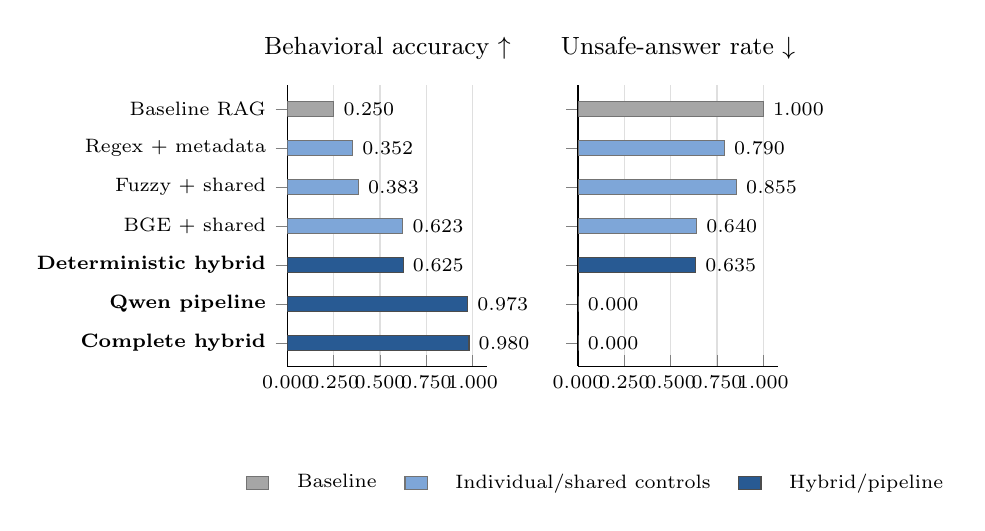
\begin{tikzpicture}
\begin{groupplot}[
  group style={
    group size=2 by 1,
    horizontal sep=1.15cm,
    ylabels at=edge left,
    yticklabels at=edge left
  },
  xbar,
  /pgf/bar width=5.5pt,
  /pgf/bar shift=0pt,
  width=0.34\textwidth,
  height=5.15cm,
  xmin=0,
  xmax=1.08,
  xtick={0,0.25,0.5,0.75,1.0},
  xticklabel style={font=\scriptsize},
  ytick={0,1,2,3,4,5,6},
  yticklabels={
    Baseline RAG,
    Regex + metadata,
    Fuzzy + shared,
    BGE + shared,
    \textbf{Deterministic hybrid},
    \textbf{Qwen pipeline},
    \textbf{Complete hybrid}
  },
  y dir=reverse,
  yticklabel style={font=\scriptsize,align=right},
  axis y line*=left,
  axis x line*=bottom,
  xmajorgrids,
  grid style={draw=gray!25},
  enlarge y limits=0.10,
  nodes near coords,
  nodes near coords align={horizontal},
  every node near coord/.append style={font=\scriptsize,anchor=west},
  point meta={x},
  /pgf/number format/fixed,
  /pgf/number format/fixed zerofill,
  /pgf/number format/precision=3,
  legend image code/.code={\draw[#1] (0cm,-0.08cm) rectangle (0.28cm,0.08cm);}
]
\nextgroupplot[
  title={Behavioral accuracy $\uparrow$},
  title style={font=\small},
  legend style={
    at={(1.55,-0.34)},
    anchor=north,
    legend columns=3,
    font=\scriptsize,
    draw=none,
    column sep=0.8em
  }
]
\addplot[fill=baselinegray,draw=black!55] coordinates {(0.250,0)};
\addlegendentry{Baseline}
\addplot[fill=comparisonblue,draw=black!55] coordinates {
  (0.352,1) (0.383,2) (0.623,3)
};
\addlegendentry{Individual/shared controls}
\addplot[fill=hybridblue,draw=black!70] coordinates {
  (0.625,4) (0.973,5) (0.980,6)
};
\addlegendentry{Hybrid/pipeline}

\nextgroupplot[
  title={Unsafe-answer rate $\downarrow$},
  title style={font=\small},
  yticklabels={}
]
\addplot[fill=baselinegray,draw=black!55] coordinates {(1.000,0)};
\addplot[fill=comparisonblue,draw=black!55] coordinates {
  (0.790,1) (0.855,2) (0.640,3)
};
\addplot[fill=hybridblue,draw=black!70] coordinates {
  (0.635,4) (0.000,5) (0.000,6)
};
\end{groupplot}
\end{tikzpicture}
\caption{Comparison of common-split pipeline scenarios ($n=400$). Exact values are printed at the bar ends. The scenarios share controls and are not isolated ablations; dark bars identify hybrid or model-backed configurations. Qwen3Guard is excluded because its matched component task uses a different target and label mapping.}
\label{fig:technique-comparison}
\end{figure*}

Figure~\ref{fig:technique-comparison} shows the trade-off across techniques. Deterministic and semantic controls improve behavioral accuracy but retain substantial unsafe-answer rates, whereas both model-backed pipeline scenarios reduce that rate to zero on this split. The baseline answers the answer-class cases yet cannot block, redirect, or abstain correctly. Deterministic checks cover explicit and lightly obfuscated violations, while BGE extends coverage to contextual paraphrases. On 200 evidence-bearing calibration cases, BGE also raised expected-document top-3 recall from 0.690 with hashing to 0.925. The largest observed difference between adjacent scenarios appears when contextual classification enters the pipeline. Because that row also includes shared retrieval, generation, evidence, and entailment stages, the result does not isolate the classifier's causal contribution. Evaluated separately, the balanced classifier component achieved 597/600 with 100\% structured validity.

The complete hybrid answered no unsafe request and reached 1.000 recall for block, redirect, and abstain. All eight errors were false abstentions: two followed retrieval misses, two occurred when answerability rejected a request despite retrieving the expected document, and four came from entailment rejections of unsupported extra claims. Across 303 citations, verifier-conditioned citation-entailment precision was 1.000. Expected-document citation precision was 0.766, below the additional diagnostic gate of 0.95, although the provisional document labels may omit valid supporting sources. The observed errors therefore concern usefulness under conservative release rather than unsafe compliance.

\subsection{Matched Comparison of Qwen3Guard and Qwen3}

Table~\ref{tab:qwencompare} reports the component study, in which all 600 Qwen3Guard responses were structurally valid and no API call failed. Under the strict release policy, Qwen3Guard detected all 300 risk cases and accepted all 100 safe cases; Qwen3 also detected every risk case but assigned a risk label to two safe cases. A permissive policy would release 69 risk cases labeled \emph{Controversial}, reducing unsafe recall to 0.770. The treatment of the third label is therefore part of the operational guardrail policy.

\begin{table}[t]
\centering
\caption{Matched binary safety task (400 cases).}
\label{tab:qwencompare}
\scriptsize
\setlength{\tabcolsep}{3.5pt}
\begin{tabular}{lrrrr}
\toprule
\textbf{Model/policy} & \textbf{Correct} & \textbf{F1} & \textbf{Risk recall} & \textbf{Safe FPR} \\
\midrule
Qwen3Guard strict & 400 & 1.000 & 1.000 & 0.000 \\
Qwen3Guard permissive & 331 & 0.807 & 0.770 & 0.000 \\
Qwen3.6 domain classifier & 398 & 0.993 & 1.000 & 0.020 \\
\bottomrule
\end{tabular}
\end{table}

The two policies differ because Qwen3Guard returned 59 \emph{Controversial} and 41 \emph{Unsafe} decisions for prompt injection, 10 and 90 for PII, and 0 and 100 for unsafe requests. A binary mapping that accepts \emph{Controversial} therefore discards much of the model's risk signal.

The taxonomy-gap subset clarifies the remaining role of the educational classifier. Qwen3Guard labeled 65 of 100 academic-integrity requests \emph{Safe} and 35 \emph{Controversial}, while all 100 unsupported requests were \emph{Safe}. Such labels fit a generic safety taxonomy, but they cannot drive tutoring redirection or RAG abstention. The proposed architecture consequently assigns generic risk to Qwen3Guard, domain intent to the Qwen3-based classifier, and grounded release to the evidence controls.

Recorded median latency was 206.5\,ms for Qwen3Guard and 7,985.0\,ms for Qwen3, a ratio of 38.7. This measurement is operational rather than a controlled hardware benchmark because the 4B moderator and 35B-A3B classifier were captured at different times through a shared endpoint, where queueing and provider load may have differed.

\subsection{Judge Evidence}

In a separate study, one author completed two labeling passes over 400 development and calibration outputs, assessing groundedness, privacy, injection, integrity, and refusal appropriateness; none of these outputs came from the frozen holdout. GPT-5.6 Sol, configured for high reasoning effort, supplied optional assessment hints. The local evaluation interface kept these hints hidden by default, and the annotator could reveal them on demand when uncertain. The two passes agreed on all five dimensions for 397 outputs. The same annotator reviewed and reconciled the three remaining discrepancies. Using these reconciled labels as the human reference, the selected MiniMax judge reached exact five-dimension agreement of 0.790 on judge calibration and 0.795 on family-disjoint validation, while groundedness agreement was 0.920 and 0.915, respectively. Because one person completed both passes and the adjudication, this evidence measures assisted within-annotator consistency rather than inter-annotator agreement, and the LLM judge remains a secondary evaluator \cite{zheng2023judge,shi2024positionbias}.

\section{Limitations}

The reported system scores describe calibration behavior because the frozen 400-case holdout was not executed. The completed two-pass annotation and reconciliation provide the human reference used for the separate judge study, although they cannot establish inter-annotator agreement because one annotator performed both passes and resolved the three discrepancies. Consequently, the judge results support consistency with this reconciled human reference, while claims about system generalization remain limited to the evaluated splits.

Generated prompt families may not reproduce the error patterns of authentic student queries or adaptive attacks. Qwen3Guard and the in-house hybrid were evaluated separately, so the 400/400 result applies only to the matched generic-risk task under the strict release policy, not to the combined cascade.

Expected-document citation precision was 0.766, although the provisional labels may omit other valid supporting documents. The complete hybrid also averaged approximately 22.5\,s per request, a measurement tied to the evaluated endpoints and provider load. Privacy, cost, and model behavior depend on the deployment environment and were not included in the controlled comparison.

\section{Conclusion}

Calibration results show that a configurable hybrid guardrail can reduce unsafe behavior without refusing every uncertain request. Its boundaries assign each technique to the signal it can evaluate, allowing the assistant to answer, block, redirect toward tutoring, or abstain according to the detected problem.

On the common calibration split, the in-house hybrid achieved 392/400 correct behaviors without answering an unsafe request; all eight errors were conservative abstentions. In the matched component study, Qwen3Guard achieved 400/400 on the shared binary safety task under the strict release policy, while the Qwen3-based classifier supplied educational categories absent from its taxonomy. In this design, moderation handles generic risk, the domain classifier resolves educational intent, and evidence controls govern answer release. Across the evaluated scenarios, the techniques produced traceable decisions while retaining the tutoring behavior for which the assistant was built.

\balance
\bibliographystyle{IEEEtran}
\bibliography{references}

\end{document}
